\documentclass[a4paper,UTF8]{article}
\usepackage{ctex}
\usepackage[margin=1.25in]{geometry}
\usepackage{color}
\usepackage{graphicx}
\usepackage{amssymb}
\usepackage{amsmath}
\usepackage{amsthm}
\usepackage{soul, color, xcolor}
\usepackage{bm}
\usepackage{tcolorbox}
\usepackage{hyperref}
\numberwithin{equation}{section}
%\usepackage[thmmarks, amsmath, thref]{ntheorem}
\theoremstyle{definition}
\newtheorem*{solution}{Solution}
\newtheorem*{prove}{Proof}
\usepackage{multirow}
\usepackage{diagbox}
\usepackage{float}

% \begin{figure}[H]
%	\centering
%	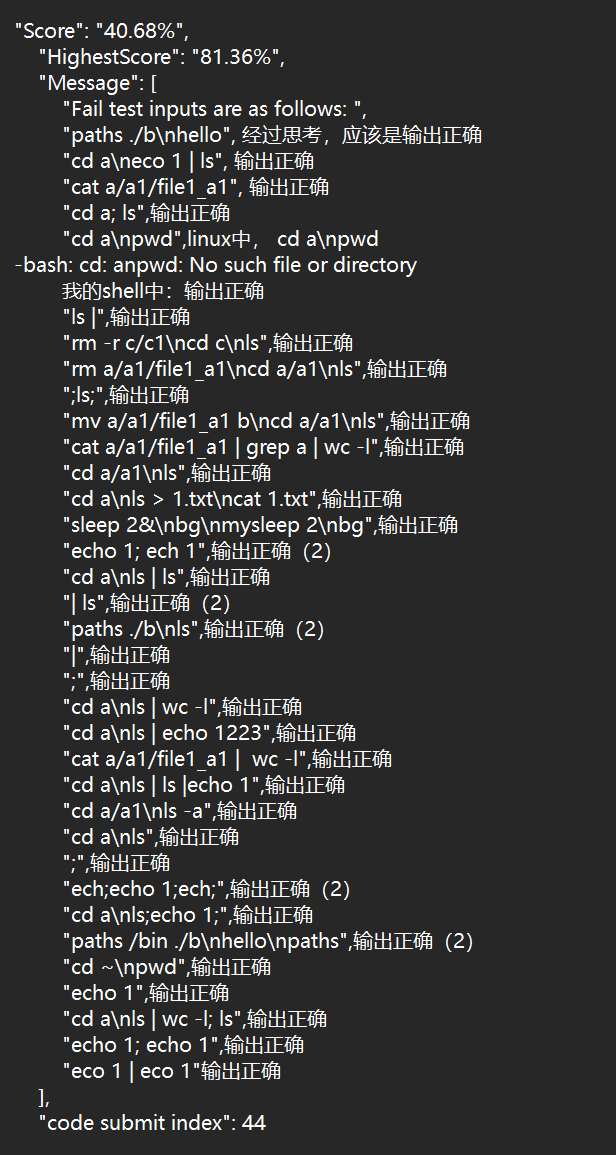
\includegraphics[width=1\textwidth]{1.png}\\
%	\caption{local test}
%	\label{fig:local test}
% \end{figure}  

\begin{document}
\title{DMA 实验报告}
\author{221300079, 王俊童, \href{mailto:221300079@smail.nju.edu.cn}{221300079@smail.nju.edu.cn}}
\maketitle

    我已经完成了dma的所有内容。

    \section{设计方案}

    介于各种涉及都需要考虑trade off 这件比较麻烦的事情,我选择first fit,即先找,找不到就compact,完了在放进去,其实基本上
    进行一次compact之后就会变得比较好看了。

    至于compact,我的思路很简单,把整个目前len有的空间里面的\#全部放到后面去,然后再把len里面的\#删掉就好了,这样既不会改变大小,也不会使得顺序发生改变.主要是利用了list的性质,再加上一些不必要的函数开销的减少。

    我的整个程序是一个O(n)时间复杂度的实现,我已经尽量把程序的空间压缩了,目前已经很小了。

    目前score:0.25
    \section{其余问题}

    正在持续改进

\end{document}